% Что пишем в программную реализацию?

% \begin{enumerate}
%   \item Раскрываем, какой язык программирования используем
%   \item Раскрываем какие библиотеки используем
%   \item Раскрываем поэтапно по шагам
% \end{enumerate}

% На каком языке программировании написано
Описанная модель реализована на языке программирования Python. Реализация сочетает достоинства применения как парадигмы ООП, так и функционального программирования за счет активного использования лямбда-выражений.

% Какую библиотеку использовали
Для реализации на языке программирования был использован внешний модуль pyomo. В части решаемой задачи этот модуль был задействован для построения математической модели и взаимодействия с решателями. Построение математической модели заключалось в динамической генерации переменных и ограничений. Взаимодействие с решателями - вызов их из переменных окружения среды, задание входных аргументов для их работы и считывание результатов вычислений.

% Про ограничения и появление 1 / M
Часть ограничений модели описана при помощизнаков строгого неравенсва. Библиотека pyomo имеет ограничения на описание ограничений. В частности устанавливает запрет на использование операторов строгого неравенства. С целью невелирования данного ограничения используется константа равная $1 / M$ - условно малое число. Тогда ограничение модели вида $x < y$ будет описано в pyomo как $x + 1 / M \le y$.

% Раскрыть применение матрешки (хоть на Бугаенко ссылаться)
С целью понижения когнитивной сложности применяемого решения и достижения управляемости поведением каждой отдельной единицы функционала весь код разбит на обособленные модули, представленные в виде классов языка программирования Python. Каждому из модулей определен перечень его зависимостей: от другого функционала или от данных. Данные в задаче представлены в виде матриц, констан и лямбда-выражений.

Компоновка их друг с другом, последовательное разрешение зависимостей происходит в едином месте - в главной функции программы. В такой схеме отсутствуют передача локальных неуправляемых параметров по цепочке вызовов в иерархии функций, а каждая отдельная единица функционала работает в своем информационном окружении.

% Привести диаграмму вызовов или uml-диаграмму
Диаграмма классов приведена на рисунке \ref{fig:uml}.

% Рисунок uml-диагараммы
\begin{figure}[H]
    \centering
    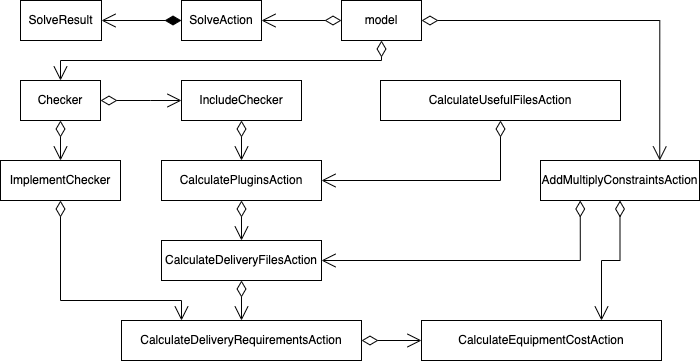
\includegraphics[width=1\textwidth]{uml}
    \caption{Диаграмма классов}
    \label{fig:uml}
\end{figure}
